% !TeX spellcheck = en_US
\section{INTRODUCTION}
\label{sec:intro}

Kuzushiji is a Japanese cursive writing style which has been used in Japan for over a thousand years, beginning in the 8th century. Over 3 millions books, on a diverse array of topics such as literature, science, mathematics and cooking are preserved today. However, the standardization of Japanese textbooks known as the “Elementary School Order” in 1900, removed Kuzushiji from regular school curriculum, as modern Japanese print became popular. As a result, most Japanese natives today cannot read books written or printed just 120 years ago, and today there are very few fluent readers of Kuzushiji (only 0.01\% of modern Japanese natives) \cite{aboutkuz}. The objective of the project, inspired by a Kaggle competition promoted by the Center for Open Data in the Humanities \cite{competition}, is building an object detection system able to transcribe pages of ancient Kuzushiji handwritten documents into contemporary Japanese characters, as shown in figure \ref{fig:objective}. Due to the lack of available human resources, there has been a great deal of interest in using machine learning to automatically recognize these historical texts and transcribe them into modern Japanese characters. Nevertheless, several challenges in Kuzushiji recognition have made the performance of existing systems extremely poor. Our deep-learning-based approach achieved notable results, with 0.77 IoU score in detection, 0.94 accuracy of classification and a 0.797 modified $F_1$ score on the competition public test set.

\begin{figure}
	\centering
	\caption{A document written in Kuzushiji whose characters have been automatically translated into modern Japanese characters.}
	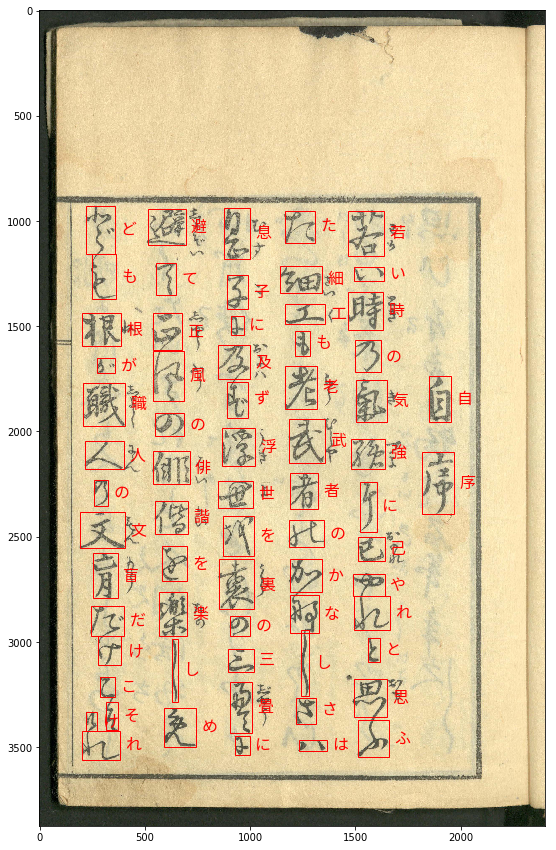
\includegraphics[width=0.6\columnwidth]{various/objective.png}
	\label{fig:objective}
\end{figure}